\chapter{aBAgalabadhx saMKeyxgaLa vagaRmUlagaLa citarx}
\vskip -30pt

$ 4,9,16,25\ldots$ muMtAda saMKeyxgaLu pUNaRvagaR saMKeyxgaLu. ivugaLige pUNaR\-vagaRmUlagaLive. Adare $2,3,5,7\ldots$ muMtAda saMKeyxgaLige pUNaRvagaRmUla\-viruvudilalx. ivelAlx aBAgalalabadhx saMKeyxgaLu. I riVtiya saMKeyxgaLige vagaRmUla\-vanunx kaMDuhiDiyalu sAdhayxvilalx. AdarU sariyAda utatxrakekx samiVpada bele\-yanunx kaMDuhiDiyabahudu.

\textbf{udAharaNege:} \qquad $2$ ra vagaRmUla
$$
\sqrt{2} = 1.41421\ldots
$$

\vspace{-0.3cm}
\noindent
$2$ ra vagaRmUlavanunx $5$ dashamAMsha sAthxnadavarege bareyalAgide. idanunx hiVgeyeV muMduvarisabahudu. I riVtiya saMKeyxgaLanunx aparimeVya saMKeyxgaLu enunxtetxVve.

peYthAgorasfna parxmeVyada parxkAra {\bf aBAgalalabadhx saMKeyxgaLa vagaRmUlavanunx} reVKAgaNitada riVti kaMDuhiDiyabahudu.

peYthAgorasfna parxmeVya namagelAlx tiLidide. 

laMbakoVna tirxBujadalilx vikaNaRda meVlina vagaRvu uLideraDu bAhugaLa vagaRgaLa motatxkekx sama.

\begin{tabular}[c]{>{$}l<{$}}
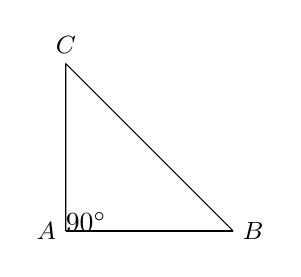
\begin{tikzpicture}[scale=1.7] %%right angle triangle
\coordinate [label=left:\small{$A$}]  (A) at (0,0);
\coordinate [label=right:\small{$B$}] (B) at (1.25,0);
\coordinate [label=above:\small{$C$}] (C) at (0,1.25);
\draw (A) -- (B);
\draw (A) -- (C);
\draw (A)--(C)-- (B);
\tkzLabelAngle[scale=0.8,pos = 0.23](C,A,B){$90^\circ$}
\end{tikzpicture}
\end{tabular}
\hspace{0.2cm}
\begin{tabular}[c]{>{$}l<{$}}
CAB\quad \text{oMdu laMbakoVna tirxBuja}\\
C\widehat{A}B = 90^{\circ}\\
CA \;\text{matutx}\; AB \;\text{oMdu seM.miV. Adare}\\ 
\text{peYthAgorasfna parxmeVyada parxkAra}
\end{tabular}

\hspace{2.1cm}
\begin{tabular}{>{$}l<{$}@{}>{$}l<{$}}
CB^2 &= CA^2+AB^2\\
     &= 1^2+1^2\\
     &= 1+1\\
CB^2 &= 2\\
\therefore CB \;\;&= \sqrt{2}
\end{tabular}

vikaNaR $CB$ ya udadxvanunx aLedAga $\sqrt{2}$ ra bele gotAtxgutatxde.

\begin{tabular}[c]{>{$}l<{$}}
\begin{tikzpicture}[scale=0.7]
    \coordinate[label=-90:\small $O$] (O) at (0,0);
    \coordinate[label=-90:\small $A$] (A) at (2,0);
    \coordinate[label=45:\small $B$] (B) at (2,2);
    \coordinate[label=90:\small $C$] (C) at (0.5,4);
    %\coordinate[label=90:$D$] (D) at (-2,4);
   %\draw [help lines](-1,0) grid(3,4);
    %\draw (O)--(B);
    \draw (O)--(A)--(B)--(C)--(O)--cycle;
 %   \draw (B)--(C)--(O);
    \draw (O)--(B)--cycle;
    %%node decleration  like  ex:1%%%
   \node [scale=0.01,label=below:\footnotesize $1$] (1) at ($ (O)!.5!(A) $) {};
   \node [scale=0.01,label=right:\footnotesize $1$] (1) at ($ (A)!.5!(B) $) {};
    \node [scale=0.01,label=above:\footnotesize $1$] (1) at ($ (C)!.5!(B) $) {};
    \node [scale=0.1,label=left:\footnotesize $\sqrt{3}$] (3) at ($ (O)!.5!(C) $) {};
   \node [scale=0.1,label=left:\footnotesize $\sqrt{2}$] (2) at ($ (O)!.6!(B) $) {};
    %%angle postion declaration%%%%%%
   \tkzLabelAngle[scale=0.8,pos = 0.50](O,A,B) {$90^\circ$}
   \tkzLabelAngle[scale=0.8,pos = -0.50](C,B,O){$90^\circ$}
\end{tikzpicture}
\end{tabular}
\hspace{0.2cm}
\begin{tabular}[c]{>{$}l<{$}}
\text{Iga}\; OBC \;\text{tirxBujadalilx}\;  \widehat{B} = 90^{\circ}\\
OB=\sqrt{2}, BC = 1 \;\text{seM.miV.}
\end{tabular}

\hspace{2.1cm}
\begin{tabular}{>{$}l<{$}@{}>{$}l<{$}}
OC^2 &= OB^2+BC^2\\
     &= (\sqrt{2})^2+(\sqrt{1})^2\\
     &=2+1\\
OC^2 &= 3\\
\therefore OC \;\;&= \sqrt{3}
\end{tabular}

$3$ oMdu aBAgalabadhx saMKeyx. adara vagaRmUlavanunx $OC$ yanunx aLeyuva mUlaka tiLiyabahudu.

\begin{tabular}[c]{>{$}l<{$}}
\begin{tikzpicture}[scale=0.6]
    \coordinate[label=-90:\small $O$] (O) at (0,0);
    \coordinate[label=-90:\small $A$] (A) at (2,0);
    \coordinate[label=45:\small $B$] (B) at (2,2);
    \coordinate[label=90:\small $C$] (C) at (0.5,4);
    \coordinate[label=90:\small $D$] (D) at (-2,4.5);
   %\draw [help lines](-4,0) grid(3,5);
    \draw (O)--(A)--(B)--(C)--(D)--cycle;
    \draw (O)--(C);
    \draw (O)--(B);
    %~ \draw (O)--(A)--(B);
    %~ \draw (O)--(D);
    %~ \draw (O)--(B);
    %~ \draw (O)--(D)--(C);
    %~ \draw (O)--(C);
    %~ \draw[line join=bevel] (B)--(C)--cycle;
    
%%node decleration  like  ex:1%%%
\node [scale=0.01,label=below:\footnotesize $1$] (1) at ($ (O)!.5!(A) $) {};
\node [scale=0.01,label=right:\footnotesize $1$] (1) at ($ (A)!.5!(B) $) {};
\node [scale=0.01,label=above:\footnotesize $1$] (1) at ($ (C)!.5!(B) $) {};
\node [scale=0.01,label=above:\footnotesize $1$] (1) at ($ (D)!.5!(C) $) {};
\node [scale=0.2,label=left: \footnotesize $\sqrt{3}$] (3) at ($ (O)!.6!(C) $) {};
\node [scale=0.3,label=left:\footnotesize $\sqrt{2}$] (2) at ($ (O)!.6!(B) $) {};
\node [scale=0.4,label=left:\footnotesize ${\sqrt{4}}$] (4) at ($ (O)!.6!(D) $) {};
%%angle postion declaration%%%%%%
\tkzLabelAngle[scale=0.8,pos = 0.60](O,A,B){\footnotesize $90^\circ$}
\tkzLabelAngle[scale=0.8,pos = -0.60](C,B,O){\footnotesize $90^\circ$}
\tkzLabelAngle[scale=0.8,pos = -0.60](D,C,O){\footnotesize $90^\circ$}
\end{tikzpicture}
\end{tabular}
\hspace{0.2cm}
\begin{tabular}[c]{>{$}l<{$}}
\text{Iga}\;OCD\; \text{tirxBujadalilx}\;\widehat{c} = 90^{\circ}\\
OC=\sqrt{3}, CD = 1 \;\text{seM.miV.}
\end{tabular}

\begin{align*}
OD^2 &= OC^2+CD^2\\
     &= (\sqrt{3})^2+(\sqrt{1})^2\\
     &=3+1\\
OD^2 &= 4\\
\therefore OD &= \sqrt{4}\\
&= 2
\end{align*}

hiVgeyeV muMduvarisidare $5,6,7,8,9,10$ ra {\bf vagaR mUlavanunx kaMDuhiDiya\-bahudu.}

meVle heVLiruva saMKeyxgaLalilx $5,6,7,8,10$ ivugaLelAlx aBAgalabadhx saMKeyxgaLu.
\begin{flalign*} 
\quad\qquad\sqrt{1}&=1.000&\\
\sqrt{2}&=1.414\\
\sqrt{3}&=1.732\\
\sqrt{4}&=2.000
\end{flalign*}

peY idoMdu aBAgalabadhxsaMKeyx. idu yAvudeV vaqtatxda paridhigU matutx vAyxsakUkx iruva parxmANa (niSapxtitx) idara bele $\frac{22}{7}$ athavA $3.1416$ ra samiVpa. idara beleyanunx tiLiyalu vishavxdAdayxMta bahaLa hiMdina dinagaLiMda parxyatanxgaLu naDedive. kirx.~sha.\ $5$ neV shatamAnadalilxdadx BAratada suparxsidadhx gaNitajacnx AyaRBaTana parxkAra idara bele sumAru $3.1416\ldots$. BAratada eraDaneya BAsakxrAcAyaRrU idara beleyanunx sumAru $3.1416$ eMdu beVroMdu riVtiyalilx lekakxhAkidAdxre. BAratada Adhunika gaNitajacnx shirxVnivAsa rAmAnujanf saha samiVkaraNada rUpadalilx idara bele tiLisidAdxre. jAyxmitiya AkaqtigaLanunx baLasi idara beleyanunx nidhaRrisalu AraMBisidAdxre. 

vijAcnxna, taMtarxjAcnxna, gaNita matutx itara keSxVtarxgaLalilx $\pi$ nunx gaNitiVya sithxra saMKeyx\-yAgi nAvu baLasutitxdedxVve. 

ameVrikAdalilx mAcfR $14$ raMdu peY dinavAgi AcarisutAtxre. $(3.14)$ yUroVpfnalilx juleY $22$ raMdu peY dinavAgi AcarisutAtxre. $(\frac{22}{7})$ beVre beVre deVshagaLalilx vividha dinagaLaMdu AcarisutAtxre.

$e$ idoMdu aBAgalabadhx saMKeyx {\rm exponential} eMba iMgilxVSf padada modala\-neya akaSxra. idara bele $2.7182\cdot$

gaNitadalilx baruva lAgaridaMge ideV AdhAra. idanunx lAgaridaMnalilx baLasidavanu jAnf neVpiyarf.

ititxVcege BwtashAsatxrX, rasAyanashAsatxrX, jiVvashAsatxrX matutx samAnavijAcnxna muMtAda keSxVtarxgaLalilx $e$ nunx baLasutAtxre.


